\documentclass{beamer}
\usepackage[UTF8]{ctex}
\usepackage{graphicx} 
\usepackage{float} 
\usepackage{subfigure}
\usepackage{algorithm,algorithmic}
\usepackage{tikzit}

\input{figs/sample.tikzstyles}
\usetheme{Madrid}
\usecolortheme{default}

%------------------------------------------------------------
%This block of code defines the information to appear in the
%Title page
\title %optional
{基于同构测试的图神经网络简介}

\author % (optional)
{吴钰同}

\date % (optional)
{\today}

%End of title page configuration block
%------------------------------------------------------------



%------------------------------------------------------------
%The next block of commands puts the table of contents at the 
%beginning of each section and highlights the current section:

\AtBeginSection[]
{
  \begin{frame}
    \frametitle{Table of Contents}
    \tableofcontents[currentsection]
  \end{frame}
}
%------------------------------------------------------------


\begin{document}

%The next statement creates the title page.
\frame{\titlepage}


%---------------------------------------------------------
%This block of code is for the table of contents after
%the title page
\begin{frame}
\frametitle{Table of Contents}
\tableofcontents
\end{frame}
%---------------------------------------------------------


\section{图同构测试}

%---------------------------------------------------------
%Changing visivility of the text
\begin{frame}

  \frametitle{图同构}

  \begin{block}{定义}
    对于两个无向图 $G$ 和 $H$,若存在它们顶点之间的双射 $f:V(G) \rightarrow V(H)$,
    使得 $G$ 中的顶点 $u$ 和 $v$ 相邻当且仅当 $H$ 中的顶点 $f(u)$ 和 $f(v)$ 相邻,
    则称 $G$ 和 $H$ 同构。
  \end{block}
  \centering
  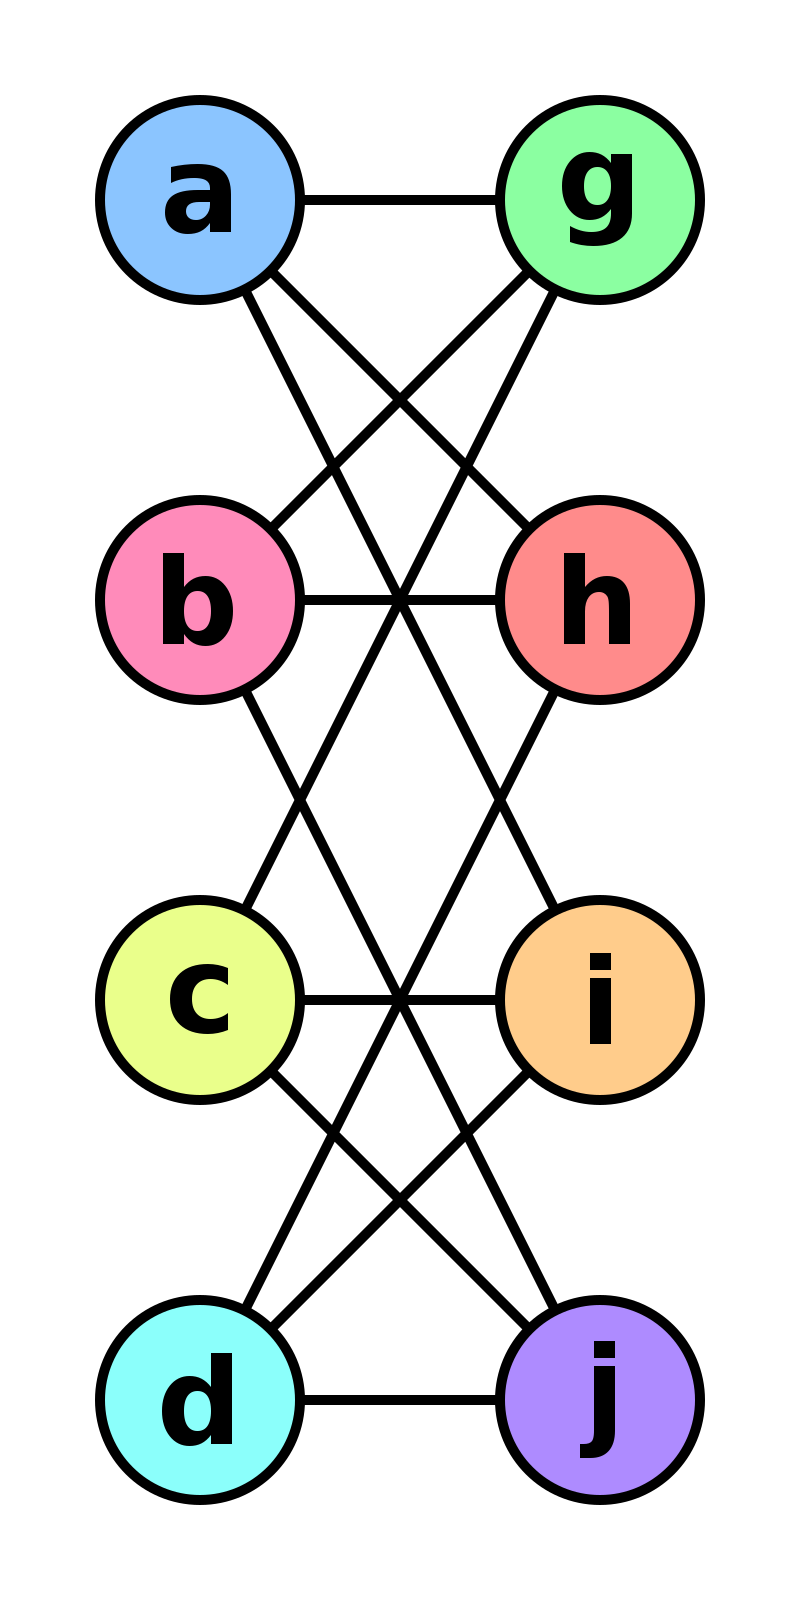
\includegraphics[scale=0.1]{figs/Graph_isomorphism_a.png}
  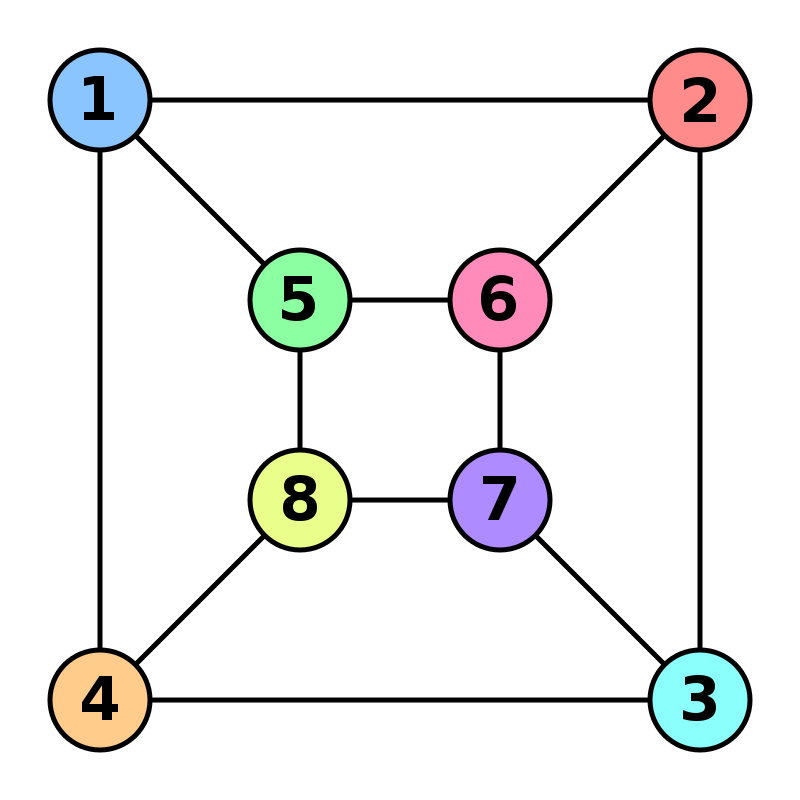
\includegraphics[scale=0.2]{figs/Graph_isomorphism_b.png}

\end{frame}

%---------------------------------------------------------


%---------------------------------------------------------
%Example of the \pause command
\begin{frame}
  \frametitle{图同构的必要不充分条件}
  \begin{center}
    \scalebox{0.8}{
      \begin{minipage}{1\linewidth}
        \begin{algorithm}[H]
        \begin{algorithmic}[1]
        \IF{$V(G) \ne V(H)$}
          \RETURN \FALSE
        \ENDIF
        \FOR{$v$ in $V(G)$ and $V(H)$}
          \STATE $L_v^0 =$ 1
        \ENDFOR
        \FOR{$i=1$ to $|V(G)|$}
          \FOR{$v$ in $V(G)$ and $V(H)$}
            \STATE $L_v^i = hash (\{ L_u^{i-1} : u \in \mathcal{N}(v) \})$
          \ENDFOR
          \IF{$\{L^i_v : v \in V(G)\} \ne \{L^i_v : v \in V(H)\}$}
            \RETURN \FALSE
          \ENDIF
          \IF{$\{L^{i-1}_v : v \in V(G)\} = \{L^i_v : v \in V(G)\}$}
            \STATE \textbf{break}
          \ENDIF
        \ENDFOR
        \RETURN \TRUE
        \end{algorithmic}
        \caption{Weisfeiler-Lehman Test}
        \label{alg:seq}
        \end{algorithm}
      \end{minipage}
      }
  \end{center}
\end{frame}
%---------------------------------------------------------

%---------------------------------------------------------
\begin{frame}

  \frametitle{Weisfeiler-Lehman Test 示例}
  \ctikzfig{figs/WL-1}

\end{frame}
%---------------------------------------------------------

%---------------------------------------------------------
\begin{frame}

  \frametitle{Weisfeiler-Lehman Test 示例}
  \ctikzfig{figs/WL-2}

\end{frame}
%---------------------------------------------------------

%---------------------------------------------------------
\begin{frame}

  \frametitle{Weisfeiler-Lehman Test 示例}
  \ctikzfig{figs/WL-3}

\end{frame}
%---------------------------------------------------------

%---------------------------------------------------------
\begin{frame}

  \frametitle{Weisfeiler-Lehman Test 示例}
  \ctikzfig{figs/WL-4}

\end{frame}
%---------------------------------------------------------

%---------------------------------------------------------
\begin{frame}

  \frametitle{Weisfeiler-Lehman Test 示例}
  \ctikzfig{figs/WL-5}

\end{frame}
%---------------------------------------------------------

%---------------------------------------------------------
\begin{frame}

  \frametitle{Weisfeiler-Lehman Test 示例}
  \ctikzfig{figs/WL-6}

\end{frame}
%---------------------------------------------------------

%---------------------------------------------------------
\begin{frame}

  \frametitle{Weisfeiler-Lehman Test 示例}
  \ctikzfig{figs/WL-7}

\end{frame}
%---------------------------------------------------------

%---------------------------------------------------------
\begin{frame}

  \frametitle{Weisfeiler-Lehman Test 示例}
  \ctikzfig{figs/WL-8}

\end{frame}
%---------------------------------------------------------

%---------------------------------------------------------
\begin{frame}

  \frametitle{Weisfeiler-Lehman Test}
  \begin{block}{WL-Test 解释}
    达到稳定时,图的标签集合是聚合运算的不动点,说明有相同标签的结点
    与其他结点有相似的邻接关系。但标签集合无法决定唯一的邻接关系。
  \end{block}
  \begin{alertblock}{WL-Test 是图同构的必要不充分条件}
    两个同构图经过上述变换后得到的标签集合一定相同,但得到相同的标签集合只能说明两个图\textbf{可能}同构。
  \end{alertblock}
  \ctikzfig{figs/WL-ce}

\end{frame}
%---------------------------------------------------------

\section{图神经网络结构}

%---------------------------------------------------------
\begin{frame}

  \frametitle{基于图数据的任务举例}
  图数据任务隐含了如下假设:结点或图的标签除了与收集的特征有关,还与图的邻接关系有关,故可以通过
  扩展 WL-Test 来设计神经网络。
  \begin{block}{结点分类}
    每个结点 $v \in V$ 都有特征向量 $x_v$ 及对应的标签 $y_v$,
    要求学习每个结点的嵌入向量 $h_v$ 和一种映射 $f$,使得结点的标签可以通过 $\hat{y}_v = f(h_v)$ 预测。
  \end{block}
  \begin{block}{图分类}
    有一系列图 $\{G_1, ..., G_N\}$ 及其标签 $\{y_1, ..., y_N\}$。
    要求学习每个图的嵌入向量 $h_G$ 和一种映射 $g$,使得图的标签可以通过 $\hat{y}_G = g(h_G)$ 预测。
  \end{block}

\end{frame}
%---------------------------------------------------------

%---------------------------------------------------------
\begin{frame}

  \frametitle{图神经网络的计算过程}
    \begin{algorithm}[H]
    \begin{algorithmic}[1]
      \FOR{$v$ in $V(G)$}
        \STATE $h_v^0 = x_v$
      \ENDFOR
      \FOR{$k=1$ to $K$}
        \STATE $a_v^k = AGGREGATE^k(\{h_u^{k-1} : u \in \mathcal{N}(v)\})$
        \STATE $h_v^k = COMBINE^k(h_v^{k-1}, a_v^k)$
      \ENDFOR
      \STATE $h_G = READOUT(\{h_v^K : v \in G\})$
    \end{algorithmic}
    \caption{GNN}
    \label{alg:gnn}
    \end{algorithm}
      
\end{frame}
%---------------------------------------------------------

%---------------------------------------------------------
\begin{frame}

  \frametitle{图神经网络的计算过程}
      
  $AGGREGATE$:聚集邻居结点的信息,如 
  $$a_v^k = MAX(\{RELU(W_a \cdot h_u^{k-1}) : u \in \mathcal{N}(v)\}).$$
  $COMBINE$:引入中心结点的信息,如
  $$h_v^k = W_c \cdot CONCAT(h_v^{k-1}, a_v^k).$$
  在卷积图神经网络中,上述两个过程合为一个:
  $$h_v^k = RELU(W \cdot MEAN \{h_u^{k-1} : u \in \mathcal{N}(v) \cup \{v\} \}).$$
  $READOUT$:聚集结点的嵌入从而生成图的嵌入,结果与输入结点的顺序无关,如按位取最大值。
\end{frame}
%---------------------------------------------------------

\section{图神经网络的表达能力}

%---------------------------------------------------------
\begin{frame}

  \frametitle{图神经网络与 WL-Test 的比较}
  \begin{block}{定理:图神经网络的表达能力不强于 WL-Test}
    设 $G_1$ 和 $G_2$ 为两个不同构的图,如果一个图神经网络 $\mathcal{A}: \mathcal{G} \rightarrow \mathbb{R}^d$
    将 $G_1$ 和 $G_2$ 映射到不同的嵌入,则 WL-Test 会认为 $G_1$ 和 $G_2$ 不同构。
  \end{block}
  \begin{block}{证明:图神经网络的表达能力不强于 WL-Test}
    以特征向量作为结点的标签,若 WL-Test 认为 $G_1$ 和 $G_2$ 同构,则每一轮迭代 $G_1$ 和 $G_2$ 都有相同的标签集合。
    
    由归纳法可证:对于任意两个结点 $u$ 和 $v$,若 WL-Test 中的标签 $L_u^i = L_v^i$,则 GNN 中的嵌入向量
    $h_u^i = h_v^i$。

    在 WL-Test 的最后一轮迭代时,$G_1$ 和 $G_2$ 具有相同的标签集合,从而说明 GNN 的结点嵌入集合是相同的,故
    GNN 的图嵌入是相同的。
  \end{block}

\end{frame}
%---------------------------------------------------------

%---------------------------------------------------------
\begin{frame}

  \frametitle{图神经网络与 WL-Test 的比较}
  \begin{block}{定理:单射图神经网络的表达能力与 WL-Test 等价}
    设 $\mathcal{A}: \mathcal{G} \rightarrow \mathbb{R}^d$ 是一个有充分多层的图神经网络,若满足如下条件:

    (1) 更新嵌入向量的过程是单射,即
    $$ h_v^k = \phi(h_v^{k-1}, f(\{h_u^{k-1} : u \in \mathcal{N}(v)\})) $$
    中的 $\phi$ 相对于两个向量输入是单射,$f$ 相对于邻居向量集合是单射。

    (2) 生成图嵌入向量的 $READOUT$ 函数相对于所有结点的向量集合 $\{h_v^k : v \in V(G)\}$ 是单射。

    则该图神经网络会把任意两个 WL-Test 判断为不同构的图映射到两个不同的嵌入向量。

  \end{block}

\end{frame}
%---------------------------------------------------------

%---------------------------------------------------------
\begin{frame}

  \frametitle{图神经网络与 WL-Test 的比较}
  \begin{block}{证明:单射图神经网络的表达能力与 WL-Test 等价}
    设 $G_1$ 和 $G_2$ 经过 $K$ 轮迭代后被 WL-Test 判断为不同构,
    $\mathcal{A}$ 使用单射函数 $\phi$ 和 $f$ 更新嵌入向量:
    $$ h_v^k = \phi(h_v^{k-1}, f(\{h_u^{k-1} : u \in \mathcal{N}(v)\})) $$
    WL-Test 使用单射哈希函数 $g$ 更新结点标签:
    $$ L_v^k = g(L_v^{k-1}, \{L_u^{k-1} : u \in \mathcal{N}(v)\}) $$
    下证:对于任意轮迭代 $k$,存在单射函数 $\varphi_k$,使得 $h_v^k = \varphi_k(L_v^k)$。

    $k = 0$ 时,$h_v^0 = L_v^0 = x_v$,故取 $\varphi_0$ 为恒等映射即可。

  \end{block}

\end{frame}
%---------------------------------------------------------

%---------------------------------------------------------
\begin{frame}

  \frametitle{图神经网络与 WL-Test 的比较}
  \begin{block}{证明:单射图神经网络的表达能力与 WL-Test 等价}
    $k \ge 1$ 时,假设第 $k - 1$ 轮迭代时存在单射函数 $\varphi_{k-1}$,则
    \begin{align*}
      h_v^k &= \phi(h_v^{k-1}, f(\{h_u^{k-1} : u \in \mathcal{N}(v)\})) \\
            &= \phi(\varphi_{k-1}(L_v^{k-1}), f(\{\varphi_{k-1}(L_u^{k-1}) : u \in \mathcal{N}(v)\})) \\
            &= \psi(L_v^{k-1}, \{L_u^{k-1} : u \in \mathcal{N}(v)\}) \\
            &= \psi \circ g^{-1} g (L_v^{k-1}, \{L_u^{k-1} : u \in \mathcal{N}(v)\}) \\
            &= \psi \circ g^{-1}(L_v^k)
    \end{align*}
    其中,$\psi = \phi \circ \varphi_{k-1}$ 为单射函数。取 $\varphi_k = \psi \circ g^{-1}$ 即证。
    
    在最后一轮迭代时,WL-Test 得到的 $G_1$ 和 $G_2$ 结点标签集合不相同,说明 $\mathcal{A}$ 得到的嵌入向量集合不相同。
    
    又由于 $READOUT$ 是单射, $G_1$ 和 $G_2$ 的图嵌入向量不相同。
  \end{block}

\end{frame}
%---------------------------------------------------------

\section{图同构神经网络}

%---------------------------------------------------------
\begin{frame}

  \frametitle{图嵌入向量的计算}
  为使图神经网络具有和 WL-Test 相同的表达能力,需要选取恰当的映射用于图嵌入向量的计算。
  该映射需要满足以下条件:
  \begin{enumerate}
    \item 当自变量是集合时是良定的,即计算结果与结点顺序无关。
    \item 是单射的,即不能把两个不同的向量集合映射到同一个向量。
    \item 是可学习的,即该映射可以表示任意单射函数。
  \end{enumerate}
  $MEAN$ 和 $MAX$ 对集合是良定的,但不是单射。
  \ctikzfig{figs/mean-max}

\end{frame}
%---------------------------------------------------------

%---------------------------------------------------------
\begin{frame}

  \frametitle{构造单射}
  \begin{block}{定理:使用求和算子能构造可数集上的单射}
    (1) 设特征集合 $\mathcal{X}$ 是可数集,则存在函数 $f: \mathcal{X} \rightarrow \mathbb{R}^n$,使得
    对于 $\mathcal{X}$ 的任意有限大小的子集 $X$,$h(X) = \sum_{x \in X} f(x)$ 是单射。

    (2) 对于任意单射函数 $g(X)$,都存在单射函数$\phi$,使得 $g(X) = \phi(\sum_{x \in X} f(x))$。
  \end{block}

  \begin{block}{证明:使用求和算子能构造可数集上的单射}
    (1) 由于 $\mathcal{X}$ 可数,故存在映射 $Z : \mathcal{X} \rightarrow \mathbb{N}$。
    又由于所有子集 $X$ 都是有限集,故存在 $N \in \mathbb{N}$,使得 $\forall X \subseteq \mathcal{X}, |X| < N$。
    取 $f(x) = N^{-Z(x)}$,则 $f(x)$ 相当于 $N$ 进制下仅小数点后 $Z(x)$ 位为 $1$ 的小数。$h(X) = \sum_{x \in X} f(x)$
    在集合意义下为单射。
    
    (2) 取 $\phi = g \circ h^{-1}$ 即可。
  \end{block}

\end{frame}
%---------------------------------------------------------

%---------------------------------------------------------
\begin{frame}

  \frametitle{图同构神经网络结构}
  \begin{block}{推论:为中心结点的嵌入添加可学习的权重}
    (1) 设特征集合 $\mathcal{X}$ 是可数集,则存在函数 $f: \mathcal{X} \rightarrow \mathbb{R}^n$,使得
    对于 $\mathcal{X}$ 的任意元素 $c$ 和有限大小的子集 $X$,$h(X) = (1 - \epsilon) \cdot f(c) + \sum_{x \in X} f(x)$ 是单射。
    
    (2) 对于任意单射函数 $g(\mathcal{N}(v))$,都存在单射函数$\varphi$,使得 $g(\mathcal{N}(v)) = \varphi((1 + \epsilon) \cdot f(h_v) + \sum_{u \in \mathcal{N}(v)} f(h_u))$.
  \end{block}
  结点嵌入的更新公式可以写为:
  \begin{align*}
    h_v^1 &= \varphi_1((1 + \epsilon_1) \cdot f_1(x_v) + \sum_{u \in \mathcal{N}(v)} f_1(x_u)) \\
    h_v^k &= \varphi_k((1 + \epsilon_k) \cdot f_k(h^{k-1}_v) + \sum_{u \in \mathcal{N}(v)} f_k(h^{k-1}_u)), k > 1.
  \end{align*}
  接下来只需想办法学习任意的 $\varphi$ 和 $f$ 即可。

\end{frame}
%---------------------------------------------------------

%---------------------------------------------------------
\begin{frame}

  \frametitle{图同构神经网络结构}
  结点嵌入的更新公式可以写为:
  \begin{align*}
    h_v^1 &= \varphi_1((1 + \epsilon_1) \cdot f_1(x_v) + \sum_{u \in \mathcal{N}(v)} f_1(x_u)) \\
    h_v^k &= \varphi_k((1 + \epsilon_k) \cdot f_k(h^{k-1}_v) + \sum_{u \in \mathcal{N}(v)} f_k(h^{k-1}_u)), k > 1.
  \end{align*}
  $k = 1$ 时,由于 $h^0 = x$ 为结点的特征向量,如果取特征向量为独热码,则 $f_1$ 为恒等映射即满足单射性。

  $k > 1$ 时,将 $f^{k} \circ \varphi^{k-1}$ 看成一个整体,使用多层感知机拟合,得到图同构神经的更新公式:
  % $$
  %   h_v^{k} = MLP^{k} ((1+\epsilon_))
  % $$
  

\end{frame}
%---------------------------------------------------------



%---------------------------------------------------------
%Highlighting text
\begin{frame}
\frametitle{Sample frame title}

In this slide, some important text will be
\alert{highlighted} because it's important.
Please, don't abuse it.

\begin{block}{Remark}
Sample text
\end{block}

\begin{alertblock}{Important theorem}
Sample text in red box
\end{alertblock}

\begin{examples}
Sample text in green box. The title of the block is ``Examples".
\end{examples}
\end{frame}
%---------------------------------------------------------


%---------------------------------------------------------
%Two columns
\begin{frame}
\frametitle{Two-column slide}

\begin{columns}

\column{0.5\textwidth}
This is a text in first column.
$$E=mc^2$$
\begin{itemize}
\item First item
\item Second item
\end{itemize}

\column{0.5\textwidth}
This text will be in the second column
and on a second tought this is a nice looking
layout in some cases.
\end{columns}
\end{frame}
%---------------------------------------------------------


\end{document}